% ==================================================
\section{פוטנציאל מדורג, פוטנציאל פעולה והולכה לאורך האקסון}
% ==================================================

\subsection{שלושה סוגי פוטנציאלים}
בנוירון קיימים שלושה סוגי שינויי מתח עיקריים:
\begin{itemize}
\item \textbf{\myen{Resting potential}} – פוטנציאל המנוחה ($V_m \approx -70\,\text{mV}$).
\item \textbf{\myen{Graded potential}} – פוטנציאל מדורג (כולל \myen{EPSP} ו-\myen{IPSP}).
\item \textbf{\myen{Action potential (AP)}} – פוטנציאל פעולה.
\end{itemize}

\begin{figure}[H]
\centering
% ודאי ששם הקובץ כאן תואם בדיוק למה שהעלית ל-Overleaf
\includegraphics[width=0.6\linewidth]{neuron_structure} 
\caption{מבנה נוירון: דנדריטים, גוף התא, \myen{axon hillock}, אקסון ומיילין}
\end{figure}

\subsection{פוטנציאל מדורג: \myen{EPSP} ו-\myen{IPSP}}
\begin{itemize}
\item \textbf{EPSP} (\myen{Excitatory postsynaptic potential}):  
דה־פולריזציה שמקרבת את הממברנה לסף העירור.
\item \textbf{IPSP} (\myen{Inhibitory postsynaptic potential}):  
היפר־פולריזציה שמרחיקה את הממברנה מהסף.
\item פוטנציאל מדורג הוא:
\begin{itemize}
\item תלוי עוצמת הגירוי.
\item דועך עם מרחק מהמקור.
\item יכול לעבור סכימה בזמן ובמרחב.
\end{itemize}
\end{itemize}

\subsection{למה נוירוטרנסמיטר לא ``מייצר'' פוטנציאל פעולה?}
נוירוטרנסמיטר נקשר לרצפטורים פוסט־סינפטיים ופותח לרוב
\textbf{תעלות תלויות־ליגנד}, ולכן הוא יוצר \textbf{פוטנציאל מדורג בלבד}.

רק אם סכימה מרחבית/זמנית של \myen{EPSP}-ים מביאה את
\textbf{\myen{axon hillock}} אל \textbf{סף העירור},
נפתחות תעלות \Na \textbf{תלויות־מתח}.

פתיחת תעלות \Na תלויות־מתח יוצרת \textbf{משוב חיובי תלוי־מתח},
שהוא התנאי ההכרחי ליצירת \textbf{פוטנציאל פעולה}.

\textbf{שורת מבחן:}  
נוירוטרנסמיטר \underline{יכול להתחיל} את התהליך,  
אבל \underline{לא מייצר בעצמו} פוטנציאל פעולה.


\subsection{פוטנציאל פעולה – גרף ושלבים}

\begin{center}
\begin{english}
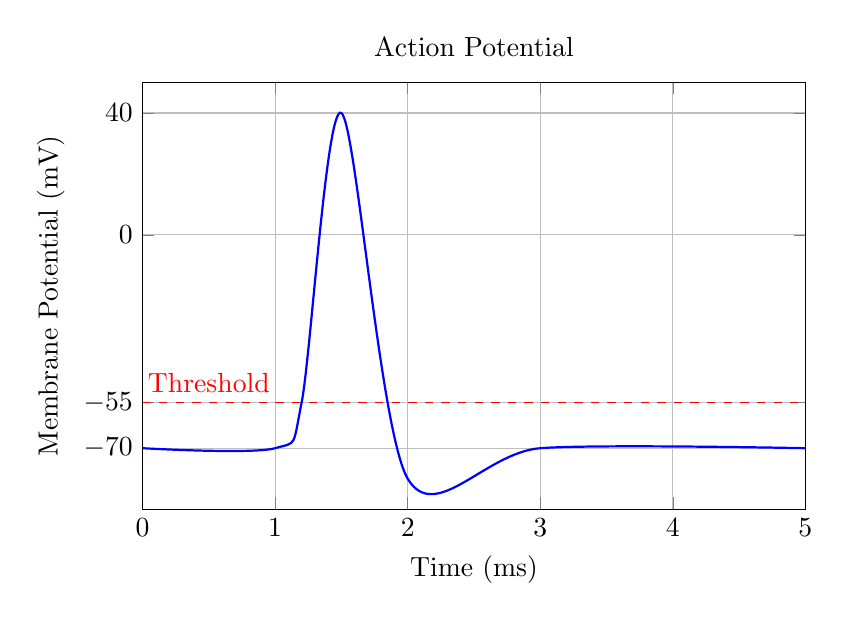
\begin{tikzpicture}
\begin{axis}[
    title={Action Potential},
    xlabel={Time (ms)},
    ylabel={Membrane Potential (mV)},
    xmin=0, xmax=5,
    ymin=-90, ymax=50,
    xtick={0,1,2,3,4,5},
    ytick={-70,-55,0,40},
    grid=major,
    width=10cm,
    height=7cm
]
\addplot[blue, thick, smooth] coordinates {
    (0,-70) (1,-70) (1.2,-55) (1.5,40) (2,-80) (3,-70) (5,-70)
};
\addplot[red, dashed] coordinates {(0,-55) (5,-55)} node[pos=0.1, above] {Threshold};
\end{axis}
\end{tikzpicture}
\end{english}
\end{center}

\subsubsection{הסטייה הקטנה לאחר ההיפר־פולריזציה}

לאחר שלב ההיפר־פולריזציה, לעיתים נצפית \textbf{סטייה קטנה וזמנית של המתח}
מעל פוטנציאל המנוחה (״גבעה קטנה״).

תופעה זו נובעת מכך ש:
\begin{itemize}
\item תעלות \Kion תלויות־מתח \textbf{אינן נסגרות בו־זמנית}.
\item סגירתן מתרחשת באופן \textbf{איטי והדרגתי}.
\item כתוצאה מכך, יציאת \Kion פוחתת בהדרגה,
והמתח יכול לעבור מעט מעל ערך המנוחה לפני התייצבות.
\end{itemize}

חשוב להדגיש:
\begin{itemize}
\item זו \textbf{אינה} פעילות סינפטית.
\item זו \textbf{אינה} פתיחת תעלות \Na.
\item זו \textbf{אינה} יצירת פוטנציאל מדורג או פעולה נוסף.
\end{itemize}

מדובר בתהליך פיזיקלי של חזרה לשיווי־משקל
הנובע מדינמיקה של תעלות יוניות.

\textbf{שורת מבחן:}  
הגבעה הקטנה לאחר ההיפר־פולריזציה נגרמת מסגירה איטית ולא סימולטנית של תעלות \Kion,
וגורמת לסטייה זמנית של המתח מעל פוטנציאל המנוחה.

\textbf{שלבי פוטנציאל הפעולה:}
\begin{itemize}
\item \textbf{\myen{Depolarization}}: פתיחת תעלות \myen{Na$^+$} תלויות־מתח \ra כניסת \myen{Na$^+$}.
\item \textbf{\myen{Repolarization}}: אינאקטיבציה של \myen{Na$^+$} + פתיחת תעלות \myen{K$^+$} \ra יציאת \myen{K$^+$}.
\item \textbf{\myen{Hyperpolarization}}: יציאת \myen{K$^+$} מוגברת \ra מתח שלילי מהרגיל.
\end{itemize}

\subsection{תקופה רפרקטורית: מוחלטת ויחסית}
\begin{itemize}
\item \textbf{תקופה רפרקטורית מוחלטת}:  
במהלך הדה־פולריזציה והרפולריזציה.  
תעלות \Na נמצאות באינאקטיבציה \ra  
\textbf{לא ניתן} לייצר פוטנציאל פעולה נוסף.
\item \textbf{תקופה רפרקטורית יחסית}:  
בשלב ההיפר־פולריזציה.  
\textbf{ניתן} לייצר פוטנציאל פעולה, אך נדרש גירוי חזק יותר.
\end{itemize}


\subsection{הולכה לאורך האקסון}
\begin{itemize}
\item פוטנציאל פעולה מתקדם \textbf{בכיוון אחד בלבד} (עקב התקופה הרפרקטורית).
\item \textbf{מיילין} \ra הולכה סלטטורית (\myen{saltatory}) בין \myen{Nodes of Ranvier}.
\item \textbf{קוטר אקסון גדול יותר} \ra התנגדות פנימית נמוכה יותר \ra מהירות הולכה גבוהה יותר.
\end{itemize}

\textbf{שורת מבחן:}  
ברגע שפוטנציאל פעולה התחיל – הוא יגיע לסוף האקסון.